% add figures from the VC paper
\chapter{Methodology}\label{ch:4}

\section{Proposed Framework}
Reviewing a variety of regional revitalization cases, we sketched a diagram at Figure 4.1 to summarize their common mechanism.
In a common case of regional revitalization, the authority makes use of local specialties and applies new ideas with technology to improve existing industry or establish a new one,
usually a tourism business, which succeeds to attract more people to visit the place and activate local economy.

We also sketched a diagram at Figure 4.2 to describe a common mechanism of regional revitalization that implements location-based AR.
In such cases, the authority applies new ideas on local features to compose unique contents for a location-based AR service,
which motivates people to access the place more, resulting in an improvement in local economy.
Despite that the contents are in digital form or accessible online, the system's location-based characteristics still make it to encourage visitors to access physically.

\begin{figure}
  \begin{minipage}{0.48\textwidth}
    \centering
    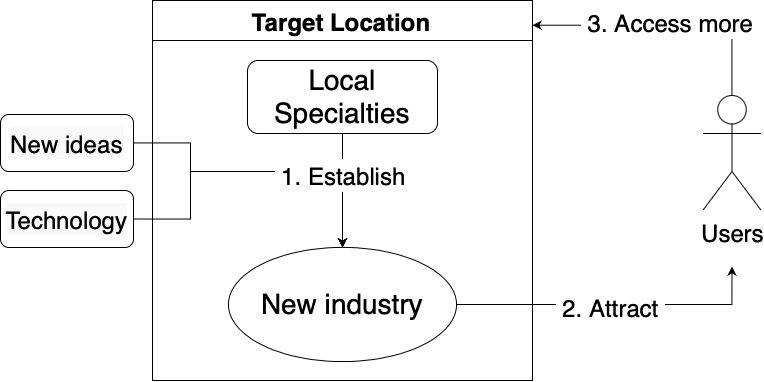
\includegraphics[width=0.9\linewidth]{resources/4_methodology/common_vitalization.png}
      \caption{Common framework of Regional Revitalization}
  \end{minipage}\hfill
  \begin{minipage}{0.48\textwidth}
    \centering
    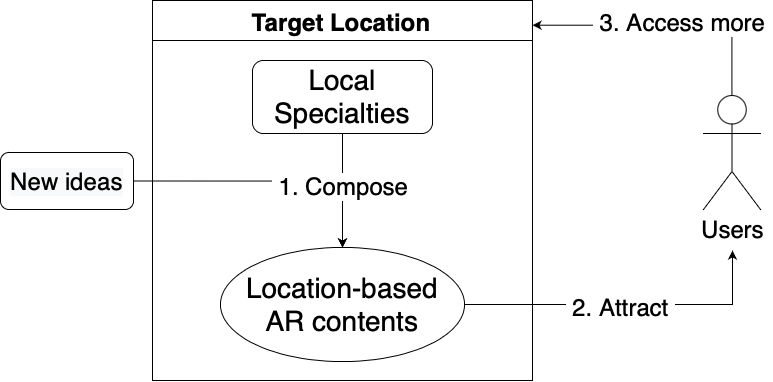
\includegraphics[width=0.9\linewidth]{resources/4_methodology/revitalization_with_AR.png}
      \caption{Framework of Regional Revitalization with location-based AR}
  \end{minipage}
\end{figure}

For places like public facilities where there is a lack of local features usable to attract visitors,
we presented a framework, sketched in Figure 4.3, that adopts a common characteristic of the places: users.
In our assumption, by enabling users to engage in co-creation of contents, which can be conducted digitally with low costs in a location-based AR system,
we anticipate that the problem of lacking usable resources becomes solvable.
Besides the issue of content creation, From Section 3.1, 3.2 and 3.3 we understand the influence on users' motivation and images about a place by both location-based AR and co-creation,
which are both included in our framework.
We also introduce a socializing mechanism to encourage users to participate in the co-creation process.
From Section 3.4 we understand that interaction between users improves people's engagement with a co-creation activity.

For this framework we proposed, we developed a prototype according to the idea of the framework, and later we examined the proposed framework with an experiment with the prototype.

\begin{figure}
  \centering
  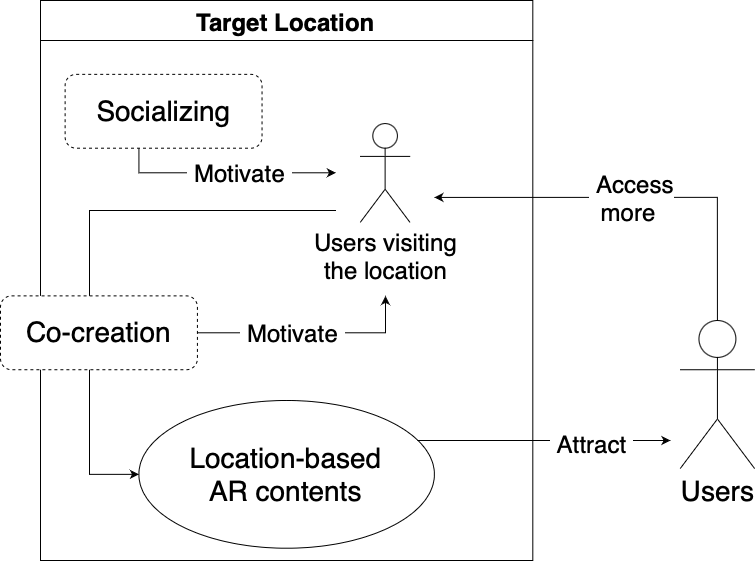
\includegraphics[width=0.8\columnwidth]{resources/4_methodology/revitalization_with_AR_and_cocreation.png}
    \caption{Proposed framework: Revitalization with location-based AR and Co-creation}
\end{figure}


\section{Prototype}
